\documentclass[14pt]{beamer}
\usepackage[T2A]{fontenc}
\usepackage[utf8]{inputenc}
\usepackage[english,russian]{babel}
\usepackage{amssymb,amsfonts,amsmath,mathtext}
\usepackage{cite,enumerate,float,indentfirst}

\graphicspath{{images/}}

\usetheme{Pittsburgh}
\usecolortheme{whale}

\setbeamercolor{footline}{fg=blue}
\setbeamertemplate{footline}{
	\leavevmode%
	\hbox{%
		\begin{beamercolorbox}[wd=.333333\paperwidth,ht=2.25ex,dp=1ex,center]{}%
			Д. В. Лазаренко, Jiji.ng
		\end{beamercolorbox}%
		\begin{beamercolorbox}[wd=.333333\paperwidth,ht=2.25ex,dp=1ex,center]{}%
			Киев, 2018
		\end{beamercolorbox}%
		\begin{beamercolorbox}[wd=.333333\paperwidth,ht=2.25ex,dp=1ex,right]{}%
			Стр. \insertframenumber{} из \inserttotalframenumber \hspace*{2ex}
		\end{beamercolorbox}}%
		\vskip0pt%
	}
	
	\newcommand{\itemi}{\item[\checkmark]}
	
	\title{\small{Рекомендательные системы и не только ...}}
	\author{
		Jiji.ng%
		\vspace{20pt}%
	}
	\date{\small{Киев, 2018}}
	
	\begin{document}
		
		\maketitle
		\begin{frame}
			\frametitle{Содержание}
			\begin{enumerate}
				\item \textbf{Постановка проблемы}
				\item \textbf{Виды рекомендательных систем}
				\begin{itemize}
					\item Content-based
					\item Collaborative Filtering
					\item Mixed models
				\end{itemize}
				\item \textbf{Photon-ml}
				\begin{itemize}
					\item Generalized Linear Model
					\item Generalized Additive Model
				\end{itemize}
				\item \textbf{Проблемы}
			\end{enumerate}
		\end{frame}
				
		\begin{frame}
			\frametitle{Постановка проблемы}
				
				$$ u \in \mathbb{U} \text{ - множество пользователей}$$ 
				$$ i \in \mathbb{I} \text{ - множество товаров}$$ 
				$$ r_{ui} \in \mathbb{Re} \text{- множество событий}$$ 	
			\begin{itemize}
				\item Offline models
				\begin{itemize}
					\item Предсказать предпочтение 
					$$ r'_{ui} = predict(u,i) \simeq r_{ui}$$
					\item Персональные рекомендации
					$$ u \longmapsto (i_1 \dots i_k) = recommend_k(u)$$
					\item Похожие объекты
					$$ u \longmapsto (i_1 \dots i_M) = similar_M(i)$$
				\end{itemize}
				\item Online models
			\end{itemize}	
		\end{frame}
		
		\begin{frame}
			\frametitle{Постановка проблемы}
			Постановка задачи звучит следующим образом: для каждого активного пользователя показать top-N объявлений с наибольшей вероятностью запроса контакта.
				\begin{figure}[h]
					\begin{minipage}[h]{0.65\linewidth}
						\center{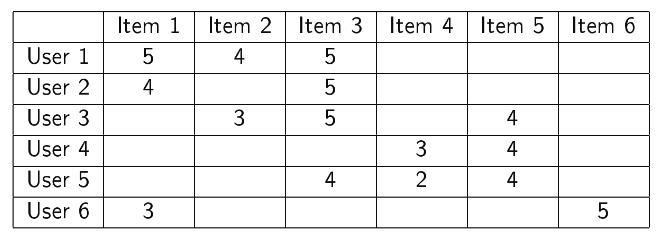
\includegraphics[width=1\linewidth]{items1}}
					\end{minipage}
					\hfill
					\begin{minipage}[h]{0.65\linewidth}
						\center{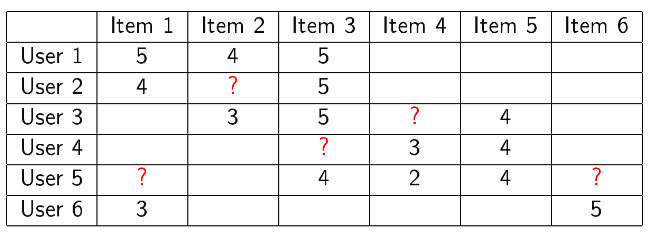
\includegraphics[width=1\linewidth]{items2}}
					\end{minipage}
				\end{figure}
		\end{frame}
		
		\begin{frame}
			\frametitle{Offline-модели}
			Offline-модели рекомендаций глобально делятся на коллаборативные и контентные. Очевидно, что каждая из этих моделей имеет свои плюсы и минусы и наилучшие результаты показывают гибридные модели, которые учитывают как историю действий пользователей, так и контент объявлений. 
		\end{frame}
		
		\begin{frame}
			\frametitle{Content-based}
			\begin{itemize}
				\item title
				\item description
				\item images
				\item ...
			\end{itemize}
			Algorithms: Latent Dirichlet allocation(LDA), relevance feedback(RF), TF-IDF  
		\end{frame}
		
		\begin{frame}
			\frametitle{Collaborative Filtering}
				Оставим в векторах только те элементы, для которых нам известны значения в обоих векторах, т.е. оставим только те продукты, которые оценили оба пользователя, или только тех пользователей, которые оба оценили данный продукт. В результате нам просто нужно определить, насколько похожи два вектора вещественных чисел.
		\end{frame}
		
		\begin{frame}
			\frametitle{Collaborative Filtering}
				Подсчитаем коэффициент корреляции:
					$ w_{ij} = \frac{\sum_a{(r_{ai}- \overline{r_i})(r_{aj}- \overline{r_i})}}{\sqrt{ \sum_a{(r_{ai}- \overline{r_i})}}{\sqrt{ \sum_a{(r_{aj}- \overline{r_j})}}}} $ \\
				где, $\overline{r_i} \text{ - средний рейтинг, выставленный пользователем i}$
		\end{frame}
		
		\begin{frame}
			\frametitle{Matrix-factorization}
			On September 21, 2009, the grand prize of US 1,000,000 was given to the BellKor's Pragmatic Chaos team which bested Netflix's own algorithm for predicting ratings by 10.06% 
			\begin{figure}[h]
				\begin{minipage}[h]{1\linewidth}
					\center{
\includegraphics[width=1\linewidth]{kaggle}}
				\end{minipage}
			\end{figure}
		\end{frame}

		\begin{frame}
			\frametitle{Matrix-factorization}
			Latent Factor Models 
				\begin{figure}[h]
					\begin{minipage}[h]{0.75\linewidth}
						\center{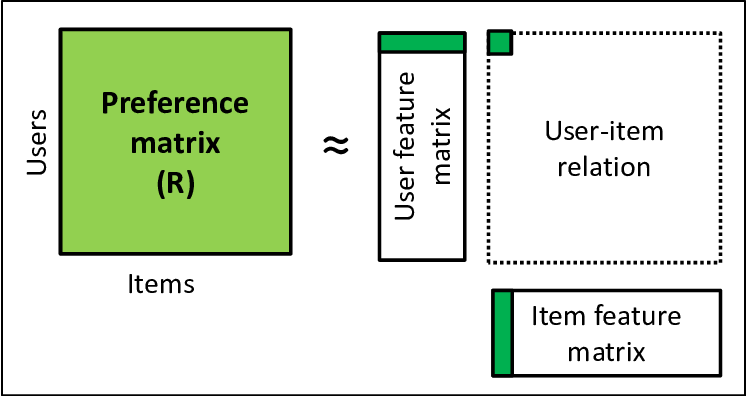
\includegraphics[width=1\linewidth]{matrix-factorization}}
					\end{minipage}
				\end{figure}
			Algorithms: Alternating least squares(ALS), Stochastic gradient descent(SGD) 
		\end{frame}
		
		\begin{frame}
			\frametitle{Matrix-factorization}
			\begin{figure}[h]
				\begin{minipage}[h]{0.75\linewidth}
					\center{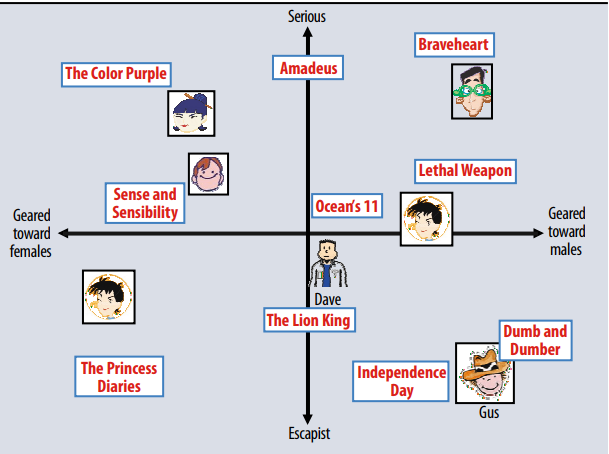
\includegraphics[width=1\linewidth]{features_space}}
				\end{minipage}
			\end{figure}
		\end{frame}
		
		\begin{frame}
			\frametitle{Photon-ml}
			\begin{figure}[h]
				\begin{minipage}[h]{1.1\linewidth}
					\center{
\includegraphics[width=1\linewidth]{linkedin}}
				\end{minipage}
			\end{figure}
		\end{frame}
		
		\begin{frame}
			\frametitle{Photon-ml}
			\begin{itemize}
				\item Generalized Linear Model (GLM)
				\item Generalized Additive Model (GAM)
				\item Generalized Additive Mixed-Effect Model(GAME)
				\item GLMix(Generalized Linear Mixed) = GLM + per-user model + per-item model
			\end{itemize}
		\end{frame}
		
		
		\begin{frame}
			\frametitle{Photon-ml}
			\begin{figure}[h]
				\begin{minipage}[h]{1.1\linewidth}
					\center{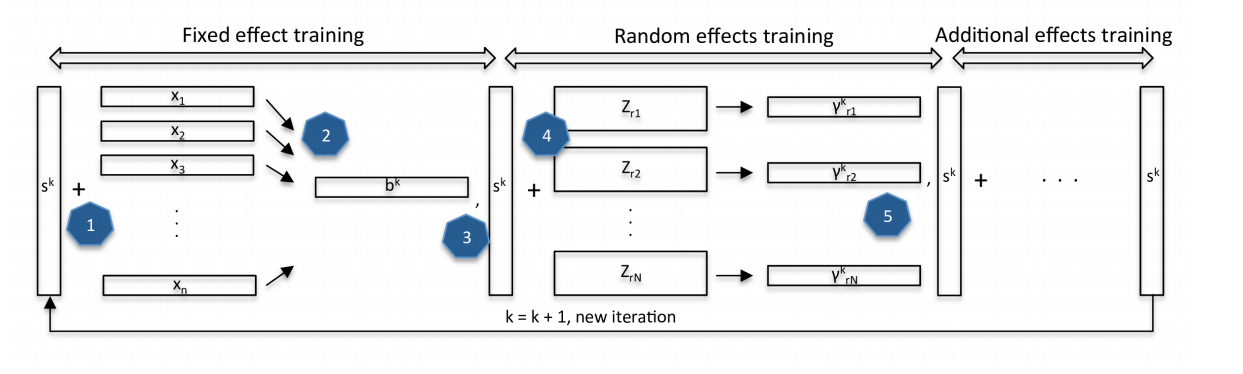
\includegraphics[width=1\linewidth]{pipline_photon}}
				\end{minipage}
			\end{figure}
			The experiments were conducted on a cluster consisting of 135 nodes managed by Apache YARN 3. Each node has 24 Intel Xeon(R) CPU E5-2640 processors with 6 cores at
			2.50GHz each, and every node has 250GB memory.
		\end{frame}
		
		\begin{frame}
			\frametitle{Evaluation}
			\begin{figure}[h]
				\begin{minipage}[h]{1.1\linewidth}
					\center{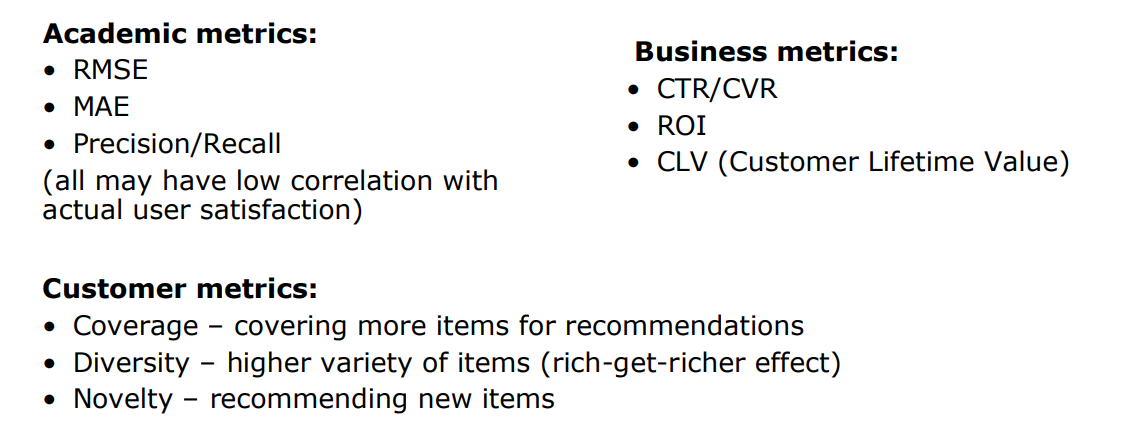
\includegraphics[width=1\linewidth]{evaluation}}
				\end{minipage}
			\end{figure}
		\end{frame}
				
		\begin{frame}
			\frametitle{Проблемы}
			\begin{itemize}
				\item Товары быстро продаются, не успев даже набрать хорошую историю по просмотрам и запросам контактов. Классические алгоритмы коллаборативной фильтрации устроены так, что объявления с короткой историей не попадают в рекомендации. Чаще рекомендуются долго живущие объявления, которые, как правило, представляют меньший интерес для покупателей.
				\item Проблемы холодного старта
				\item Как заставить это все быстро работать
			\end{itemize}
		\end{frame}

		\begin{frame}
		\frametitle{Проблемы}
				\begin{figure}[h]
					\begin{minipage}[h]{0.2\linewidth}
						\center{
\includegraphics[width=1\linewidth]{spark}}
					\end{minipage}
					\begin{minipage}[h]{0.3\linewidth}
						\center{
\includegraphics[width=1\linewidth]{hadoop}}
					\end{minipage} \\
					\begin{minipage}[h]{0.2\linewidth}
						\center{
\includegraphics[width=1\linewidth]{hive}}
					\end{minipage}
					\begin{minipage}[h]{0.2\linewidth}
						\center{
\includegraphics[width=1\linewidth]{elastic}}
					\end{minipage}
				\end{figure}
		\end{frame}

		\begin{frame}
			\begin{center}
				Спасибо за внимание!
			\end{center}
		\end{frame}
		
	\end{document} 